\chapter{Hilbert空间}\vspace{-2em}

欧几里得空间 ${\mathbb{R}}^{n}$ 配备了自然的内积 $\langle  \cdot  , \cdot  \rangle$ .该内积具有多方面用途:

\begin{itemize}
\item 它定义了欧几里得范数 $\| \bm{x}\|  \doteq  \sqrt{\langle \bm{x},\bm{x}\rangle }$ .
\item 它确定了正交空间与正交投影，并允许我们构造彼此正交的向量基 $\left\{  {{\bm{v}}_{1},\ldots ,{\bm{v}}_{n}}\right\}$.得益于内积，计算向量 $\bm{v} \in  {\mathbb{R}}^{n}$ 关于正交基的分量变得十分简便.
\item 每个线性泛函 $\varphi  : {\mathbb{R}}^{n} \mapsto  \mathbb{R}$ 均可表示为内积形式: $\varphi \left( \bm{x}\right)  = \langle \bm{w},\bm{x}\rangle$ ，其中 $\bm{w} \in  {\mathbb{R}}^{n}$ 为某个适当的向量.
\item 有了内积，便可定义一类对称算子，其具有诸多良好性质.我们回顾:若对所有 $x,y \in  {\mathbb{R}}^{n}$ 均有 $\langle A\bm{x},\bm{y}\rangle  = \langle \bm{x},A\bm{y}\rangle$ ，则称 $A : {\mathbb{R}}^{n} \mapsto  {\mathbb{R}}^{n}$ 为对称算子.在 ${\mathbb{R}}^{n}$ 的标准基下，对称算子对应于对称 $n \times  n$ 矩阵.
\item 始终依赖内积，可定义一类正算子.我们回顾:若对所有 $\bm{x} \in  {\mathbb{R}}^{n},\bm{x} \neq  0$ 均有 $\langle A\bm{x},\bm{x}\rangle  > 0$ ，则 $A : {\mathbb{R}}^{n} \mapsto  {\mathbb{R}}^{n}$ 是严格正定的.此时，映射 $\bm{x} \mapsto  \langle A\bm{x},\bm{x}\rangle$ 是一个正定二次型.
\end{itemize}

本章目标是展示欧几里得内积的定义与性质如何推广至无限维向量空间.

\section{具有内积的空间}

\begin{definition}[内积空间]
    设 $H$ 是域 $\mathbb{K}$ (实数域或复数域)上的向量空间，$H$ 上的一个内积是指映射 $\left( {\cdot , \cdot  }\right):H\times H\to\mathbb{K}$，并满足如下性质:对任意 $x,y,z \in  H$ 与 $\alpha  \in  \mathbb{K}$ ，均有
    \begin{enumerate}[(i)]
        \item  $\left( {x,y}\right)  = \overline{\left( y,x\right) }$ ，其中上横线表示复共轭；
        \item $\left( {x + y,z}\right)  = \left( {x,z}\right)  + \left( {y,z}\right)$ ；
        \item $\left( {{\alpha x},z}\right)  = \alpha \left( {x,z}\right)$
        \item $\left( {x,x}\right)  \geq  0$ ，且等号成立当且仅当 $x = 0$ .
    \end{enumerate}
\end{definition}



注意，上述性质还蕴含
\begin{equation}\tag{5.1}\label{eq:inner-product-linearity}
\left( {x,y + z}\right)  = \left( {x,y}\right)  + \left( {x,z}\right) ,\;\left( {x,{\alpha y}}\right)  = \overline{\alpha }\left( {x,y}\right) .
\end{equation}

当 $\mathbb{K} = \mathbb{R}$ 时，性质 (i)-(iii) 单纯表明:实向量空间上的内积是一个对称双线性映射.关联上述内积，我们还定义
\begin{equation}\tag{5.2}\label{eq:norm-from-inner-product}
\| x\|  \doteq  \sqrt{\left( x,x\right) }.
\end{equation}

后文证明的Minkowski不等式表明，这确为向量空间 $H$ 上的一个范数.

\begin{theorem}[两个基本不等式]\label{thm:basic-inequalities}
设 $H$ 是具有内积 $\left( {\cdot , \cdot  }\right)$ 的向量空间，则

(i) $\left| \left( {x,y}\right) \right|  \leq  \| x\| \| y\| \;$ (Cauchy-Schwartz不等式)；

(ii) $\| x + y\|  \leq  \| x\|  + \| y\| \;$ (Minkowski不等式).
\end{theorem}

\begin{proof}
(i) 若 $y = 0$ ，第一个不等式显然成立.为涵盖一般情形，令
\[
a \doteq  \left( {x,x}\right) ,\;b \doteq  \left( {x,y}\right) ,\;c \doteq  \left( {y,y}\right) .
\]

对任一标量 $\lambda  \in  \mathbb{K}$ ，均有
\[
0 \leq  \left( {x + {\lambda y},x + {\lambda y}}\right)  = a + b\overline{\lambda } + \bar{b}\lambda  + {c\lambda }\overline{\lambda }.
\]

取 $\lambda  =  - b/c$ ，得
\[
0 \leq  a - \frac{b\bar{b}}{c}.
\]

由于 $c = \left( {y,y}\right)  > 0$ ，两边同乘 $c$ ，得
\[
0 \leq  {ac} - {\left| b\right| }^{2} = \| x{\| }^{2}\| y{\| }^{2} - {\left| \left( x,y\right) \right| }^{2},
\]

即证 (i).

\noindent (ii) 由Schwartz不等式，
\[
\operatorname{Re}\left( {x,y}\right)  \leq  \left| \left( {x,y}\right) \right|  \leq  \| x\| \| y\|
\]

因此
{\setjot[-2]\begin{align*}
    \| x + y{\| }^{2} &= \left( {x + y,x + y}\right)  = \| x{\| }^{2} + \| y{\| }^{2} + 2\operatorname{Re}\left( {x,y}\right)\\
    &\leq  \| x{\| }^{2} + \| y{\| }^{2} + 2\| x\| \| y\| \\
    &= {\left( \| x\|  + \| y\| \right) }^{2}.
\end{align*}}


取平方根即得 (ii).
\end{proof}

\begin{definition}[Hilbert空间]
    配备内积 $\left( {\cdot , \cdot  }\right)$ 的向量空间 $H$ ，若关于范数 $\| x\|  \doteq  \sqrt{\left( x,x\right) }$ 完备，则称为\colorbf{Hilbert空间}.
\end{definition}


\begin{instance}\label{ins:euclidean-space-hilbert}
具有内积 $\left( {x,y}\right)  = {x}_{1}{y}_{1} + \; \cdots  + {x}_{n}{y}_{n}$ 的欧几里得空间 ${\mathbb{R}}^{n}$ 是实数域上的Hilbert空间.
\end{instance}

\begin{instance}\label{ins:l2-hilbert}
所有满足 $x = \; \left( {{x}_{1},{x}_{2},\ldots }\right)$ 的复数序列构成的空间 ${\ell }^{2}$ ，
\[
\| x\|  = {\left( \sum\limits_{{k = 1}}^{\infty }{\left| {x}_{k}\right| }^{2}\right) }^{1/2} < \infty
\]
是复数域上的Hilbert空间，其内积为
\[
\left( {x,y}\right)  \doteq  \sum\limits_{{k = 1}}^{\infty }{x}_{k}\overline{{y}_{k}}.
\]
\end{instance}

\begin{instance}\label{ins:L2-omega-hilbert}
设 $\Omega  \subseteq  {\mathbb{R}}^{n}$ 为任意开集.所有平方可积映射 $f : \Omega  \mapsto  \mathbb{R}$ 构成的空间 ${L}^{2}\left( {\Omega ;\mathbb{R}}\right)$ 是Hilbert空间，其中
\[
\left( {f,g}\right)  \doteq  {\int }_{\Omega }f\left( x\right) g\left( x\right) {dx},\;\| f{\| }_{{L}^{2}} \doteq  {\left( {\int }_{\Omega }{\left| f\left( x\right) \right| }^{2}dx\right) }^{1/2}
\]
\end{instance}

\section{正交投影}

对任意子集 $S \subseteq  H$ ，记 $\operatorname{span}\left( S\right)$ 为 $S$ 中元素的所有有限线性组合构成的集合，即
\begin{equation}\tag{5.3}\label{eq:span-def}
\operatorname{span}\left( S\right)  \doteq  \left\{  {\sum\limits_{{i = 1}}^{N}{c}_{i}{x}_{i};N \geq  1,{c}_{i} \in  \mathbb{K},{x}_{i} \in  S}\right\}  .
\end{equation}

一般地， $\operatorname{span}\left( S\right)$ 是 $H$ 的一个子空间，但未必闭.其闭包 $V \doteq  \overline{\operatorname{span}\left( S\right) }$ 称为由 $S$ 生成的空间，由此可引入完全集的概念.
\begin{definition}[完全集]
    一个集合$S$是\colorbf{完全集}，当且仅当其满足以下任一等价条件：
    \begin{enumerate}[(i)]
        \item $S$ 生成整个空间 $H$，即$\overline{\operatorname{span}\left( S\right) }=H$.
        \item $S$是无孤立点的闭集，即对每个 $x \in  H$ ，存在元素序列 ${x}_{n} \in  \operatorname{span}\left( S\right)$ ，使得 $\norm{{x}_{n} - x} \rightarrow  0$ (当 $n \rightarrow  \infty .$ ).
    \end{enumerate}
\end{definition}

\begin{definition}[正交]
    Hilbert空间 $H$ 中两个元素 $x,y$ 称为\colorbf{正交的}，若 $\left( {x,y}\right)  = 0$ .
\end{definition}

对任意子集 $S \subseteq  H$ ，其\bluebf{正交子空间}定义为
\[
{S}^{ \bot  } \doteq  \{ y \in  H;\left( {y,x}\right)  = 0\forall\,x \in  S\} .
\]

注意: ${S}^{ \bot  }$ 恒为 $H$ 的闭子空间.

\begin{theorem}[正交投影]\label{thm:orthogonal-projection}
设 $H$ 为 Hilbert 空间， $V \subseteq  H$ 为其一闭子空间.则

(i) $H = V \oplus  {V}^{ \bot  }$ ，即每个 $x \in  H$ 可唯一表示为 $x = y + z$ ，其中 $y \in  V$ 且 $z \in  {V}^{ \bot  }$ .

(ii) $y \doteq  {P}_{V}\left( x\right)$ 是 $V$ 中到 $x$ 距离最小的唯一点，而 $z \doteq  {P}_{{V}^{ \bot  }}\left( x\right)$ 是 ${V}^{ \bot  }$ 中到 $x$ 距离最小的唯一点.

(iii) 正交投影算子 $P_V:x \mapsto {P}_{V}(x)\doteq y$ 与 $P_{V^{\perp}}:x \mapsto  {P}_{{V}^{ \bot  }}\left( x\right)\doteq z$ 均为线性连续算子，其范数为 $\leq  1$ .
\end{theorem}

\begin{figure}[htbp]
\centering
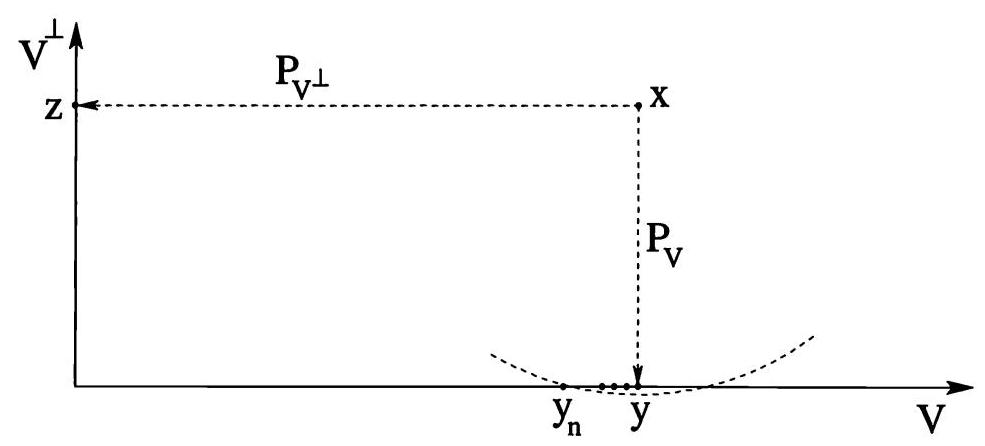
\includegraphics[width=0.9\textwidth]{images/bo_d6ik6nn7aajc739ct1l0_92_246_1195_985_446_0.jpg}
\caption{在子空间 $V$ 及其正交补子空间 ${V}^{ \bot  }$ 上构造正交投影.}
\label{fig:orthogonal-projection}
\end{figure}

\begin{proof}
1. 给定 $x \in  H$ ，我们首先证明存在唯一的点 $y \in  V$ ，其到 $x$ 的距离最小.令
\[
\alpha  \doteq  d\left( {x,V}\right)  \doteq  \mathop{\inf }\limits_{{y \in  V}}\| x - y\| .
\]

则存在点列 ${\left( {y}_{n}\right) }_{n \geq  1}$ ，使得 $\mathop{\lim }\limits_{{n \rightarrow  \infty }}\norm{x - {y}_{n}} = \; \alpha$ .我们断言 ${\left( {y}_{n}\right) }_{n \geq  1}$ 是 Cauchy 列.事实上，对任意两点 $u,v \in  H$ ，有
\[
\| u + v{\| }^{2} + \| u - v{\| }^{2} = 2\| u{\| }^{2} + 2\| v{\| }^{2}.
\]

将此等式应用于 $u = x - {y}_{m}$ 与 $v = x - {y}_{n}$ ，得
\begin{equation}\tag{5.4}\label{eq:projection-cauchy-bound}
{\norm{y}_{m} - {y}_{n}}^{2} = 2{\norm{x} - {y}_{m}}^{2} + 2{\norm{x} - {y}_{n}}^{2} - 4{\norm{x} - \frac{{y}_{m} + {y}_{n}}{2}}^{2}.
\end{equation}

由于 $\frac{{y}_{m} + {y}_{n}}{2} \in  V$ ，故 ${\norm{x} - \frac{{y}_{m} + {y}_{n}}{2}}^{2} \geq  {\alpha }^{2}$ .因此
{\setjot[-2]\begin{align*}
    \mathop{\limsup }\limits_{{m,n \rightarrow  \infty }}{\norm{y}_{m} - {y}_{n}}^{2} &\leq  2\mathop{\limsup }\limits_{{m \rightarrow  \infty }}{\norm{x} - {y}_{m}}^{2} + 2\mathop{\limsup }\limits_{{n \rightarrow  \infty }}{\norm{x} - {y}_{n}}^{2}\\
    &\;\;\;- 4\mathop{\liminf }\limits_{{m,n \rightarrow  \infty }}{\norm{x} - \frac{{y}_{m} + {y}_{n}}{2}}^{2} \\
    &\leq  2{\alpha }^{2} + 2{\alpha }^{2} - 4{\alpha }^{2} = 0
\end{align*}}

证毕.

\noindent 2. 因 $V$ 是闭的(从而完备)，序列 ${\left( {y}_{n}\right) }_{n \geq  1}$ 收敛于唯一极限 $y$ ，且满足 $\| x - y\|  = d\left( {x,V}\right)$.我们断言该点唯一:若对另一点 $\norm{x - {y}^{\prime }} = d\left( {x,V}\right)$ 亦有 ${y}^{\prime }$ ，则同式\eqref{eq:projection-cauchy-bound}中所用论证可得
\[
{\norm{y} - {y}^{\prime }}^{2} = 2{\norm{x} - y}^{2} + 2{\norm{x} - {y}^{\prime }}^{2} - 4{\norm{x} - \frac{y + {y}^{\prime }}{2}}^{2} \leq  2{\alpha }^{2} + 2{\alpha }^{2} - 4{\alpha }^{2},
\]

因为 $\frac{y + {y}^{\prime }}{2} \in  V$ .故 ${y}^{\prime } = y$ .这表明映射 $x \mapsto  {P}_{V}\left( x\right)$ 定义良好.

\noindent 3. 我们现证明 ${P}_{V}\left( x\right)$ 亦可表征为满足下式的唯一一点 $y \in  V$ :
\begin{equation}\tag{5.5}\label{eq:projection-orthogonality}
x - y \in  {V}^{ \bot  }\text{ . }
\end{equation}

任取向量 $v \in  V$ .由步骤 1，对 $\lambda  \in  \mathbb{R}$ ，实值映射
\[
\lambda \; \mapsto  \;{\norm{x} - \left( y + \lambda v\right) }^{2} = {\norm{x} - y}^{2} + {\left| \lambda \right| }^{2}\| v{\| }^{2} + 2\operatorname{Re}\left( {x - y,\;{\lambda v}}\right)
\]

在 $\lambda  = 0$ 处取得其唯一的全局最小值.因此，其在 $\lambda  = 0$ 处的导数必为零.这已证明对每个 $v \in  V$ 均有 $\operatorname{Re}\left( {x - y,v}\right)  = 0$ .若 $H$ 是复Hilbert空间，则可用 $v$ 替换 $- {iv}$，并同样得出 $\operatorname{Im}\left( {x - y,v}\right)  = \operatorname{Re}\left( {x - y, - {iv}}\right)  = 0$ .这就证明了\eqref{eq:projection-orthogonality}.

\noindent 4. 接下来，我们证明满足 $x - y \in  {V}^{ \bot  }$ 的点 $y \in  V$ 是唯一的.事实上，若 ${y}^{\prime } \in  V$ 是另一个满足 $x - {y}^{\prime } \in  {V}^{ \bot  }$ 的点，则
\[
{\norm{y} - {y}^{\prime }}^{2} = \left( {y - {y}^{\prime },y - {y}^{\prime }}\right)  = \left( {y - {y}^{\prime },x - {y}^{\prime }}\right)  - \left( {y - {y}^{\prime },x - y}\right)  = 0
\]

因为 $y - {y}^{\prime } \in  V$ ，而 $x - {y}^{\prime } \in  {V}^{ \bot  }$ 且 $x - y \in  {V}^{ \bot  }$ .

\noindent 5. 最后，我们证明正交投影 ${P}_{V} : H \mapsto  V$ 是一个范数为 $\norm{P}_{V} \leq  1$ 的线性算子.

若 $y = {P}_{V}\left( x\right)$ 且 ${y}^{\prime } = {P}_{V}\left( {x}^{\prime }\right)$ ，则对任意标量 $\alpha ,{\alpha }^{\prime } \in  \mathbb{K}$ ，均有
\[
{\alpha y} + {\alpha }^{\prime }{y}^{\prime } \in  V,\;{\alpha x} + {\alpha }^{\prime }{x}^{\prime } - \left( {{\alpha y} + {\alpha }^{\prime }{y}^{\prime }}\right)  \in  {V}^{ \bot  }.
\]

由第 3 步可知，这足以推出 ${P}_{V}\left( {{\alpha x} + {\alpha }^{\prime }{x}^{\prime }}\right)  = {\alpha y} + {\alpha }^{\prime }{y}^{\prime }$ ，从而证明投影算子 ${P}_{V}$ 是线性的.类似地，算子 ${P}_{{V}^{ \bot  }} = \; I - {P}_{V}$ 也是线性的.

由于向量 ${P}_{V}\left( x\right)$ 与 ${P}_{{V}^{ \bot  }}\left( x\right)  = x - {P}_{V}\left( x\right)$ 正交，根据勾股定理有
\[
{\norm{P}_{V}\left( x\right) }^{2} + {\norm{x} - {P}_{V}\left( x\right) }^{2} = \| x{\| }^{2}.
\]

这证明了 $\norm{P}_{V} \leq  1$ 与 $\norm{P}_{{V}^{ \bot  }} \leq  1$ .
\end{proof}

\begin{remark}\label{rem:projection-norm}
在前述定理中，若 $V \neq  \{ 0\}$ ，则 $\norm{P}_{V} = 1$ ；若 $V \neq  H$ ，则 $\norm{P}_{{V}^{ \bot  }} = 1$ .
\end{remark}

\section{Hilbert空间上的线性泛函}

下一个定理表明，Hilbert空间可与其对偶空间等同.换言之，每个元素 $x \in  H$ 确定一个有界线性泛函 ${\phi }^{x} : H \mapsto  \mathbb{K}$ ，定义为 ${\phi }^{x}\left( y\right)  = \left( {y,x}\right)$ ；反之， $H$ 上的每个有界线性泛函均具有形式 $y \mapsto  \left( {y,x}\right)$ ，其中 $x \in  H$ 为某个元素.

\begin{theorem}[线性泛函的Riesz表示]\label{thm:riesz-representation-functional}
设 $H$ 为一个Hilbert空间.

(i) 对每个 $x \in  H$ ，映射 $y \mapsto  \left( {y,x}\right)$ 是 $H$ 上的一个连续线性泛函.

(ii) 设 $y \mapsto  {Ay}$ 为 $H$ 上的一个连续线性泛函，则存在唯一元素 $\bm{a} \in  H$ ，使得对每个 $y \in  H$ 均有 ${Ay} = \left( {y,\bm{a}}\right)$ .
\end{theorem}

\begin{proof}
(i) 设给定 $x \in  H$ .由内积定义，映射 ${\phi }^{x}$ (定义为 ${\phi }^{x}\left( y\right)  \doteq  \left( {y,x}\right)$ )是线性的.该线性映射的有界性由Cauchy-Schwartz不等式得出:
\[
\norm{\phi }^{x} \doteq  \mathop{\sup }\limits_{{\| y\|  \leq  1}}\left| \left( {y,x}\right) \right|  \leq  \mathop{\sup }\limits_{{\| y\|  \leq  1}}\| y\| \| x\|  = \| x\| .
\]

(ii) 反之，设给定一线性连续泛函 $y \mapsto  {Ay}$ .若对所有 $y \in  H$ 均有 ${Ay} \equiv  0$ ，则结论显然成立，取 $\bm{a} = \bm{0}$ (即 $H$ 中的零向量)即可.

\begin{figure}[htbp]
\centering
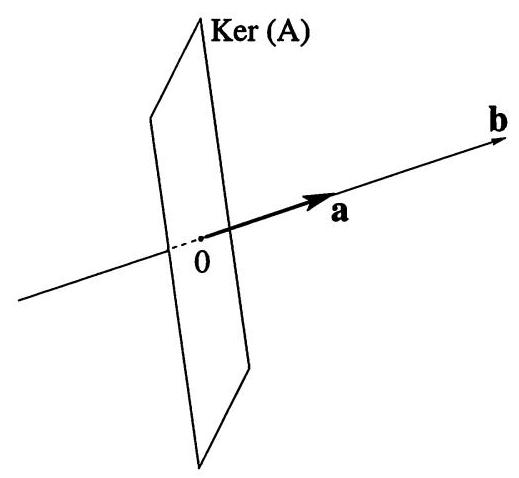
\includegraphics[width=0.4\textwidth]{images/bo_d6ik6nn7aajc739ct1l0_95_483_252_519_478_0.jpg}
\caption{若对每个 $y$ 均有 ${Ay} = \left( {y,\bm{a}}\right)$ ，则向量 a 必与 $\operatorname{Ker}\left( A\right)$ 正交.由于 ${\left(  \operatorname{Ker}\left( A\right) \right)  }^{ \bot  }$ 是一维的，对任意非零向量 $\bm{b} \in  {\left(  \operatorname{Ker}\left( A\right) \right)  }^{ \bot  }$ ，必有 $\bm{a} = t\bm{b}$ ，其中数 $t$ 由恒等式 $A\bm{b} = \left( {\bm{b},t\bm{b}}\right)$ 确定.}
\label{fig:riesz-representation-geometry}
\end{figure}

否则， $V \doteq  \operatorname{Ker}\left( A\right)$ 是一个闭超平面.其正交补 ${V}^{ \bot  }$ 是一个一维子空间.任取一非零向量 $\bm{b} \in  {V}^{ \bot  }$ ，并定义 $\kappa  = A\bm{b}/\| \bm{b}{\| }^{2},\bm{a} \doteq  \overline{\kappa }\bm{b}$ .此选择给出
\begin{equation}\tag{5.6}\label{eq:riesz-key-identity}
0 \neq  A\bm{b} = \kappa \left( {\bm{b},\bm{b}}\right)  = \left( {\bm{b},\overline{\kappa }\bm{b}}\right)  = \left( {\bm{b},\bm{a}}\right) .
\end{equation}

对任意向量 $y \in  H$ ，可将 $y$ 分解为一个属于 $V$ 的向量与属于${V}^{ \bot  }$ 的向量之和:
\[
y = {P}_{V}\left( y\right)  + \alpha \bm{b}
\]

其中 $\alpha  \in  \mathbb{K}$ 为某元素.由\eqref{eq:riesz-key-identity}立即得
\begin{align*}
    {Ay} &= A\left( {{P}_{V}\left( y\right) }\right)  + A\left( {\alpha \bm{b}}\right)  = 0 + {\alpha A}\bm{b} = 0 + \alpha \left( {\bm{b},\bm{a}}\right) \\
    &= \left( {{P}_{V}\left( y\right) ,\bm{a}}\right)  + \left( {\alpha \bm{b},\bm{a}}\right)  = \left( {y,\bm{a}}\right) .
\end{align*}


\end{proof}

\begin{remark}\label{rem:hilbert-dual-identification}
设 $H$ 为实数域上的Hilbert空间.由前述定理，映射 $x \mapsto  {\phi }^{x}$ 是 $H$ 与其对偶空间 ${H}^{ * }$ (即 $H$ 上所有有界线性泛函构成的空间)之间的等距同构.因此，我们可将两个空间 $H$ 与 ${H}^{ * }$ 等同看待.

若此时 $\Lambda  : H \mapsto  H$ 是有界线性算子，则其伴随算子 ${\Lambda }^{ * } : {H}^{ * } \mapsto \; {H}^{ * }$ 可被识别为算子 ${\Lambda }^{ * } : H \mapsto  H$ .该伴随算子由如下恒等式刻画
\[
\left( {x,{\Lambda }^{ * }y}\right)  = \left( {{\Lambda x},y}\right) \;\forall\,x,y \in  H.
\]
\end{remark}

\section{Gram-Schmidt正交化}

设 $H$ 为Hilbert空间.若向量 $x \in  H$ 满足 $\| x\|  = 1$ ，则称其为\bluebf{单位化的}.
\begin{definition}[标准正交]
    设$H$是Hilbert空间，子集 $E \subset  H$ 称为\colorbf{标准正交的}，当且仅当 $E$ 中每个向量的范数均为1，且 $E$ 中任意两个向量彼此正交.
\end{definition}


接下来，考虑有限个线性无关向量构成的集合 $S = \left\{  {{v}_{1},{v}_{2},\ldots ,{v}_{n}}\right\}$ .假设 $x \in  \operatorname{span}\left\{  {{v}_{1},\ldots ,{v}_{n}}\right\}$ ，于是有
\[
x = \sum\limits_{{k = 1}}^{n}{\theta }_{k}{v}_{k}
\]
对某些系数 ${\theta }_{k}$ 成立.为实际计算这些系数，我们注意到:对每个 $j = 1,\ldots ,n$ ，必有
\[
\left( {x,{v}_{j}}\right)  = \sum\limits_{{k = 1}}^{n}{\theta }_{k}\left( {{v}_{k},{v}_{j}}\right) .
\]

因此，数 ${\theta }_{1},\ldots ,{\theta }_{n}$ 可通过求解 $n$ 个线性方程组成的方程组得到
\begin{equation}\tag{5.7}\label{eq:gram-schmidt-linear-system}
\left( \begin{matrix} \left( {{v}_{1},{v}_{1}}\right) & & \left( {{v}_{n},{v}_{1}}\right) \\  \vdots &  \ddots  & \vdots \\  \left( {{v}_{1},{v}_{n}}\right) & \cdots & \left( {{v}_{n},{v}_{n}}\right)  \end{matrix}\right) \left( \begin{matrix} {\theta }_{1} \\  \vdots \\  {\theta }_{n} \end{matrix}\right)  = \left( \begin{matrix} \left( {x,{v}_{1}}\right) \\  \vdots \\  \left( {x,{v}_{n}}\right)  \end{matrix}\right) .
\end{equation}

当矩阵为对角阵(即对所有 $i \neq  j$ 均有 $\left( {{v}_{i},{v}_{j}}\right)  = 0$ )时，该方程组更易求解.这恰好发生在向量 ${v}_{1},{v}_{2},\ldots ,{v}_{n}$ 彼此正交时.此时显式解为
\[
{\theta }_{k} = \frac{\left( x,{v}_{k}\right) }{\left( {v}_{k},{v}_{k}\right) }.
\]

在集合 $\left\{  {{v}_{1},\ldots ,{v}_{n}}\right\}$ 为标准正交的特殊情形下(即对每个 $j = 1,\ldots ,n$ 均有 $\left( {{v}_{j},{v}_{j}}\right)  =$ = 1)，上述公式进一步简化为
\[
{\theta }_{k} = \left( {x,{v}_{k}}\right) .
\]

前述分析表明:若已有标准正交基可用，则计算将变得简便得多.现给定一个(有限或可数的)线性无关集 $S = \left\{  {{v}_{1},{v}_{2},\ldots }\right\}$ ，我们描述一种通用方法，以构造标准正交集 $\left\{  {{e}_{1},{e}_{2},\ldots }\right\}$ ，使得
\[
{E}_{n} \doteq  \operatorname{span}\left\{  {{e}_{1},\ldots ,{e}_{n}}\right\}   = \operatorname{span}\left\{  {{v}_{1},\ldots ,{v}_{n}}\right\}
\]

对每个 $n \geq  1$ 均成立.该构造将通过归纳法实现.

\subsection{Gram-Schmidt正交化算法}

(i) 首先定义 ${e}_{1} \doteq  \frac{{v}_{1}}{\norm{v}_{1}}$ .

(ii) 若已构造出 ${e}_{1},\ldots ,{e}_{n - 1}$ ，令 ${\widetilde{v}}_{n}$ 为 ${v}_{n}$ 在子空间 ${E}_{n - 1} = \operatorname{span}\left\{  {{v}_{1},\ldots ,{v}_{n - 1}}\right\}   = \operatorname{span}\left\{  {{e}_{1},\ldots ,{e}_{n - 1}}\right\}$ 上的垂直投影，然后定义
\begin{equation}\tag{5.8}\label{eq:gram-schmidt-en-def}
{e}_{n} \doteq  \frac{{v}_{n} - {\widetilde{v}}_{n}}{\norm{v}_{n} - {\widetilde{v}}_{n}}.
\end{equation}

注意 ${v}_{n} \neq  {\widetilde{v}}_{n}$ ，因为 ${v}_{n} \notin  \operatorname{span}\left\{  {{v}_{1},\ldots ,{v}_{n - 1}}\right\}$ .故 ${e}_{n}$ 定义良好且范数为1.此外， ${e}_{n}$ 与所有向量 ${e}_{1},\ldots ,{e}_{n - 1}$ 均正交.

注意， ${v}_{n}$ 在子空间 ${E}_{n - 1}$ 上的投影由下式计算:
\[
{\widetilde{v}}_{n} = \sum\limits_{{k = 1}}^{{n - 1}}\left( {{v}_{n},{e}_{k}}\right) {e}_{k}
\]

由式\eqref{eq:gram-schmidt-en-def}，这给出显式公式
\[
{e}_{n} = \frac{{v}_{n} - \sum\limits_{{k = 1}}^{{n - 1}}\left( {{v}_{n},{e}_{k}}\right) {e}_{k}}{\norm{v}_{n} - \sum\limits_{{k = 1}}^{{n - 1}}\left( {v}_{n},{e}_{k}\right) {e}_{k}}.
\]

\begin{figure}[htbp]
\centering
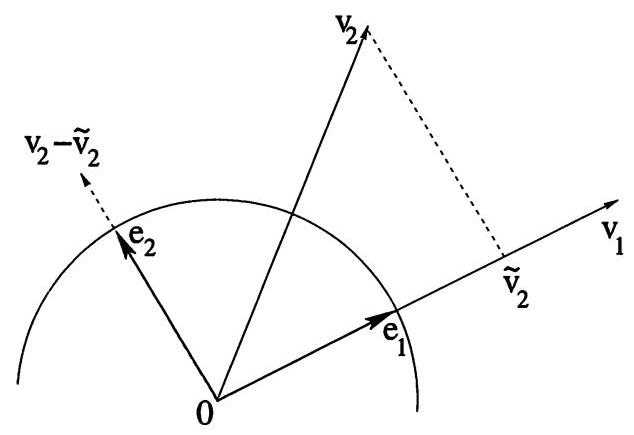
\includegraphics[width=0.6\textwidth]{images/bo_d6ik6nn7aajc739ct1l0_97_408_1210_634_435_0.jpg}
\caption{Gram-Schmidt正交化过程，应用于两个向量 ${v}_{1},{v}_{2}$.}
\label{fig:gram-schmidt-process}
\end{figure}

\section{标准正交集}

若 $\left\{  {{e}_{1},{e}_{2},\ldots ,{e}_{n}}\right\}$ 是 ${\mathbb{R}}^{n}$ 的一组标准正交基，则任意向量 $x \in  {\mathbb{R}}^{n}$ 均可唯一地表示为如下线性组合:
\[
x = \sum\limits_{{k = 1}}^{n}\left( {x,{e}_{k}}\right) {e}_{k}
\]

注意，每一项 $\left( {x,{e}_{k}}\right) {e}_{k}$ 表示向量 $x$ 在由 ${e}_{k}$ 张成的一维子空间上的垂直投影.

在无穷维Hilbert空间 $H$ 中，上述有限和应替换为无穷级数.对许多应用而言，理解该级数在何种条件下收敛、以及何时达到等式至关重要.
\begin{equation}\tag{5.9}\label{eq:orthonormal-expansion}
x = \sum\limits_{{k \geq  1}}\left( {x,{e}_{k}}\right) {e}_{k}
\end{equation}

\begin{lemma}[正交子空间的性质]\label{lem:orthogonal-subspace-properties}
设 $H$ 为一个Hilbert空间.对任意子集 $S \subseteq  H$ ，其正交子空间 ${S}^{ \bot  }$ 是 $H$ 的一个闭子空间.此外，下列命题等价:
\begin{enumerate}[(i)]
    \item $\operatorname{span}\left( S\right)$ 在 $H$ 中稠密.
    \item ${S}^{ \bot  } = \{ 0\}$ .
\end{enumerate}
\end{lemma}

\begin{proof}
1. ${S}^{ \bot  }$ 是 $H$ 的子空间，这一点显然成立.现设 ${x}_{n} \in  {S}^{ \bot  }$ 与 ${x}_{n} \rightarrow  x$ 属于 $n \rightarrow  \infty$ ，则对每个 $a \in  S$ ，有
\[
\left( {x,a}\right)  = \mathop{\lim }\limits_{{n \rightarrow  \infty }}\left( {{x}_{n},a}\right)  = 0.
\]

因此 $x \in  {S}^{ \bot  }$ 亦属其中，表明该子空间是闭的.

\noindent 2. 为证明蕴含关系 (i) $\Rightarrow$ (ii)，假设 $\operatorname{span}\left( S\right)$ 在 $H$ 中稠密，并设 $x \in  {S}^{ \bot  }$ ，因此对每个 $a \in  S$ 均有 $\left( {x,a}\right)  = 0$ .于是存在一列线性组合，记为
\[
{x}_{n} = \sum\limits_{{k = 1}}^{{N}_{n}}{\theta }_{n,k}{a}_{n,k}
\]

其中 ${a}_{n,k} \in  S$ ，且当 $n \rightarrow  \infty$ 时有 ${x}_{n} \rightarrow  x$ .这意味着
{\begin{align*}
    \left( {x,x}\right)  &= \lim_{{n \rightarrow  \infty }}\left( {x,{x}_{n}}\right)  = \lim_{{n \rightarrow  \infty }}\left( {x,\sum_{{k = 1}}^{{N}_{n}}{\theta }_{n,k}{a}_{n,k}}\right)\\
    &=\lim_{n \rightarrow  \infty }\sum_{{k = 1}}^{{N}_{n}}{\theta }_{n,k}\left( {x,{a}_{n,k}}\right)  = 0,
\end{align*}}

从而得出 $x = 0$ .

\noindent 3. 为证明蕴含关系 (ii) $\Rightarrow$ (i)，设 $V$ 为 $\operatorname{span}\left( S\right)$ 的闭包.若 (i) 不成立，则 $V \neq  H$ ，且存在某个元素 $y \notin  V$ .考虑正交投影 ${P}_{V}\left( y\right)$ .于是 $w \doteq  y - {P}_{V}\left( y\right)$ 是一个非零向量，且垂直于 $V$ .由于 $w \in  {S}^{ \bot  }$ ，这与 (ii) 矛盾.
\end{proof}

给定一个标准正交序列，下述定理给出级数\eqref{eq:orthonormal-expansion}的收敛性，并刻画其和.

\begin{theorem}[正交级数的和]\label{thm:orthogonal-series-sum}
设 $S = \left\{  {{e}_{1},{e}_{2},\ldots }\right\}$ 为Hilbert空间 $H$ 中一个(有限或可数的)标准正交集.令 $V$ 为由 $S$ 生成的闭子空间，并记 ${P}_{V} : H \mapsto  V$ 为其垂直投影.则对任意的$x \in  H$ ，均有Bézier不等式
\begin{equation}\tag{5.10}\label{eq:bessel-inequality}
\sum\limits_{{k \geq  1}}{\left| \left( x,{e}_{k}\right) \right| }^{2} = {\norm{P}_{V}x}^{2} \leq  \| x{\| }^{2}.
\end{equation}

此外，
\begin{equation}\tag{5.11}\label{eq:orthogonal-series-sum}
\sum\limits_{{k \geq  1}}\left( {x,{e}_{k}}\right) {e}_{k} = {P}_{V}x
\end{equation}

\end{theorem}

\begin{proof}
1. 对任意 $n \geq  1$ ，记为 ${V}_{n} \doteq  \operatorname{span}\left\{  {{e}_{1},\ldots ,{e}_{n}}\right\}$ .则
\[
{P}_{{V}_{n}}x = \sum\limits_{{k = 1}}^{n}\left( {x,{e}_{k}}\right) {e}_{k}
\]

因此，由标准正交性可得
{\begin{align*}
    {\norm{P}_{{V}_{n}}x}^{2}& = \left( {\sum\limits_{{j = 1}}^{n}\left( {x,{e}_{j}}\right) {e}_{j},\sum\limits_{{k = 1}}^{n}\left( {x,{e}_{k}}\right) {e}_{k}}\right)  = \sum\limits_{{k,j = 1}}^{n}\left( {x,{e}_{j}}\right) \overline{\left( x,{e}_{k}\right) }\left( {{e}_{j},{e}_{k}}\right)\\
    &= \sum\limits_{{k = 1}}^{n}{\left| \left( x,{e}_{k}\right) \right| }^{2}.
\end{align*}}

由于对每个 $n$ 均有 $\norm{{P}_{{V}_{n}}x} \leq  \| x\|$ ，故不等式\eqref{eq:bessel-inequality}得证.

\noindent 2. 若集合 $S$ 有限，则恒等式\eqref{eq:orthogonal-series-sum}显然成立.为涵盖 $S$ 可数的情形，我们首先证明部分和序列
\[
{x}_{n} \doteq  \sum\limits_{{k = 1}}^{n}\left( {x,{e}_{k}}\right) {e}_{k}
\]
是Cauchy列.事实上，级数\eqref{eq:orthogonal-series-sum}中所有项彼此正交.对 $m < n$ ，利用勾股定理及\eqref{eq:bessel-inequality}可得
\[
{\norm{x}_{n} - {x}_{m}}^{2} = \sum\limits_{{k = m + 1}}^{n}{\left| \left( x,{e}_{k}\right) \right| }^{2} \rightarrow  0,\;m,n \rightarrow  \infty .
\]

由于$H$完备，故存在$\widetilde{x}$ ，使得部分和${x}_{n} \rightarrow  \widetilde{x}$ ，即该极限即为级数\eqref{eq:orthogonal-series-sum}之和.

\noindent 3. 为完成证明，需验证 $\widetilde{x} = {P}_{V}x$ .

由于对每个 $n \geq  1$ 和 ${x}_{n} \rightarrow  \widetilde{x}$ 均有 ${x}_{n} \in  V$ ，显然 $\widetilde{x}$ 属于闭子空间 $V$ .此外，
\[
\left( {x - \widetilde{x},{e}_{k}}\right)  = \mathop{\lim }\limits_{{n \rightarrow  \infty }}\left( {x - {x}_{n},{e}_{k}}\right)  = 0
\]

因为一旦 $n \geq  k$ 成立，便有 $\left( {x - {x}_{n},{e}_{k}}\right)  = 0$ .这表明 $x - \widetilde{x}$ 与所有向量 ${e}_{k}$ 均正交，从而亦与这些向量的任意线性组合正交.因此， $x - \widetilde{x}$ 与每个向量 $v \in  V$ 正交.性质 $\widetilde{x} \in  V$ 与 $x - \widetilde{x} \in  {V}^{ \bot  }$ 共同推出 $\widetilde{x} = {P}_{V}x$ .
\end{proof}

\begin{definition}[标准正交基]
    若标准正交集 $S\subset  H$满足$\operatorname{span}\left( S\right)$ 在 $H$ 中稠密，则称$S$为\colorbf{标准正交基}.
\end{definition}
此时，由 $S$ 生成的闭子空间即为 $V = H$ .因而对每个 $x \in  H$ 均有 ${P}_{V}x = x$ ，且由\eqref{eq:bessel-inequality}--\eqref{eq:orthogonal-series-sum}可得
\begin{equation}\tag{5.12}\label{eq:parseval-identity}
\sum\limits_{{k \geq  1}}{\left| \left( x,{e}_{k}\right) \right| }^{2} = \| x{\| }^{2},\;\sum\limits_{{k \geq  1}}\left( {x,{e}_{k}}\right) {e}_{k} = x.
\end{equation}

\subsection{傅里叶级数}
作为前述理论的一个应用，考虑复值函数构成的Hilbert空间 ${L}^{2}\left( {\left(  {-\pi ,\pi }\right)  ;\mathbb{C}}\right)$ ，其内积定义为
\begin{equation}\tag{5.13}\label{eq:L2-inner-product-Fourier}
\left( {f,g}\right)  \doteq  {\int }_{-\pi }^{\pi }f\left( x\right) \overline{g\left( x\right) }{dx}.
\end{equation}

在此空间中，函数集
\[
{\varphi }_{n}\left( x\right)  \doteq  \frac{{e}^{inx}}{\sqrt{2\pi }},\;n \in  \mathbb{Z},
\]
是标准正交的.事实上，
\[
{\int }_{-\pi }^{\pi }{e}^{imx}\overline{{e}^{inx}}{dx} = {\int }_{-\pi }^{\pi }{e}^{i\left( {m - n}\right) x}{dx} = \begin{cases} 0 &m \neq  n, \\  {2\pi } &m = n. \end{cases}
\]

我们断言：
\begin{theorem}[$L^2((-\pi,\pi))$的标准正交基]
    可数集$S \doteq  \left\{  {{e}^{inx};n \in  \mathbb{Z}}\right\}$ 是 ${L}^{2}\left( \left(  {-\pi ,\pi }\right)  \right)$ 的一个标准正交基.
\end{theorem}
\begin{proof}
为证 $S$ 稠密，任取函数 $f \in  {L}^{2}\left( {\left(  {-\pi ,\pi }\right)  ;\mathbb{C}}\right)$ .对任意 $\varepsilon  > 0$ ，存在连续函数 ${f}_{\varepsilon } : \left(  {-\pi ,\pi }\right)   \mapsto  \mathbb{C}$ ，使得
\begin{equation}\tag{5.14}\label{eq:L2-approx-continuous-periodic}
{\norm{f}_{\varepsilon } - f}_{{L}^{2}\left( \left(  {-\pi ,\pi }\right)  \right) } < \varepsilon ,\;{f}_{\varepsilon }\left( {-\pi }\right)  = {f}_{\varepsilon }\left( \pi \right) .
\end{equation}
反之，如第3章例3.8所示，我们可以找到一个如下形式的复三角多项式
\[
p\left( x\right)  = \sum\limits_{{k =  - N}}^{N}{\alpha }_{k}{e}^{ikx}
\]

使得
\begin{equation}\tag{5.15}\label{eq:uniform-trig-approx}
{\norm{f}_{\varepsilon } - p}_{{\mathcal{C}}^{0}\left( \left(  {-\pi ,\pi }\right)  \right) } \doteq  \mathop{\max }\limits_{{x \in  \left(  {-\pi ,\pi }\right)  }}\left| {{f}_{\varepsilon }\left( x\right)  - p\left( x\right) }\right|  < \varepsilon .
\end{equation}

注意到
\[
{\norm{f}_{\varepsilon } - p}_{{L}^{2}} = {\left( {\int }_{-\pi }^{\pi }{\left| {f}_{\varepsilon }\left( x\right)  - p\left( x\right) \right| }^{2}dx\right) }^{1/2} \leq  \sqrt{2\pi }{\norm{f}_{\varepsilon } - p}_{{\mathcal{C}}^{0}},
\]

显然， ${f}_{\varepsilon }$ 也可按 ${L}^{2}$ 范数被三角多项式 $p\left( \cdot \right)$ 逼近.结合\eqref{eq:L2-approx-continuous-periodic}与\eqref{eq:uniform-trig-approx}，我们得出 $\overline{\operatorname{span}\left( S\right) } = {L}^{2}\left( \left(  {-\pi ,\pi }\right)  \right)$ .
\end{proof}



现在考虑复三角级数
\begin{equation}\tag{5.16}\label{eq:complex-fourier-series}
\sum\limits_{{k =  - \infty }}^{\infty }{a}_{k}\frac{{e}^{ikx}}{\sqrt{2\pi }},\;{a}_{k} \doteq  \left( {f,{\varphi }_{k}}\right)  = {\int }_{-\pi }^{\pi }f\left( x\right) \frac{{e}^{-{ikx}}}{\sqrt{2\pi }}{dx}.
\end{equation}

由前述定理可知，该级数在 ${L}^{2}\left( \left(  {-\pi ,\pi }\right)  \right)$ 中收敛于 $f$ ，即
\begin{equation}\tag{5.17}\label{eq:fourier-L2-convergence}
\mathop{\lim }\limits_{{N \rightarrow  \infty }}{\norm{f} - \sum\limits_{{k =  - N}}^{N}{a}_{k}{\varphi }_{k}}_{{L}^{2}\left( \left(  {-\pi ,\pi }\right)  \right) } = 0.
\end{equation}

该结果可重述为
\begin{corollary}\label{cor:fourier-L2-convergence}
设 $f \in  {L}^{2}\left( {\left(  {-\pi ,\pi }\right)  ;\mathbb{C}}\right)$ 是一个复值、平方可和的函数.定义系数
\[
{c}_{k} \doteq  \frac{1}{2\pi }{\int }_{-\pi }^{\pi }f\left( y\right) {e}^{-{iky}}{dy}
\]

则有如下收敛性
\[
\mathop{\lim }\limits_{{N \rightarrow  \infty }}{\int }_{-\pi }^{\pi }{\left| f\left( x\right)  - \sum\limits_{{k =  - N}}^{N}{c}_{k}{e}^{ikx}\right| }^{2}{dx} = 0.
\]
\end{corollary}

\section{正定算子}

线性代数的一个基本问题是求解线性方程组
\[
A\bm{x} = \bm{b},
\]
其中 $A$ 是一个 $n \times  n$ 矩阵， $\bm{b}$ 是 ${\mathbb{R}}^{n}$ 中的一个向量.保证解存在且唯一的条件之一是 $A$ 严格正定.事实上，若内积满足对每个 $x \neq  0$ 均有 $\langle A\bm{x},\bm{x}\rangle  > 0$ ，则 $A$ 必为满秩.因此上述线性方程组存在唯一解.本节将证明，该结论在无穷维Hilbert空间中依然成立.

\begin{definition}\label{def:strictly-positive-definite-operator}
设 $H$ 是一个实数域上的Hilbert空间.称线性算子 $A : H \mapsto  H$ 为严格正定\footnotemark，若存在 $\beta  > 0$ ，使得
\begin{equation}\tag{5.18}\label{eq:strictly-positive-definite}
\left( {{Au},u}\right)  \geq  \beta \| u{\| }^{2}\;\forall\,u \in  H.
\end{equation}
\end{definition}
\footnotetext{{在文献中，满足不等式\eqref{eq:strictly-positive-definite}的算子通常称为严格单调算子.此处我们更倾向称之为严格正定算子，以强调其与线性代数中正定矩阵的联系.}}

\begin{theorem}[正定算子的逆]\label{thm:inverse-positive-definite-operator}
设 $H$ 是一个实Hilbert空间， $A : H \mapsto  H$ 是一个有界线性算子，且严格正定，即满足\eqref{eq:strictly-positive-definite}.则对任意 $f \in  H$ ，存在唯一 $u \doteq  {A}^{-1}f \in  H$ ，使得
\begin{equation}\tag{5.19}\label{eq:positive-definite-inverse-equation}
{Au} = f.
\end{equation}

逆算子 ${A}^{-1}$ 满足
\begin{equation}\tag{5.20}\label{eq:positive-definite-inverse-bound}
\norm{A}^{-1} \leq  \frac{1}{\beta }.
\end{equation}

\end{theorem}

\begin{proof}
在假设\eqref{eq:strictly-positive-definite}下，需证连续映射 $A$ 是单射且满射.

\noindent 1. 由\eqref{eq:strictly-positive-definite}可得
\[
\beta \| u{\| }^{2} \leq  \left( {{Au},u}\right)  \leq  \| {Au}\| \| u\| .
\]

因此
\begin{equation}\tag{5.21}\label{eq:positive-definite-beta-bound}
\beta \| u\|  \leq  \| {Au}\| .
\end{equation}

若 ${Au} = 0$ ，则 $u = 0$ ，从而证得 $\operatorname{Ker}\left( A\right)  = \{ 0\}$ 且 $A$ 是单射.

\noindent 2. 接下来，我们声称 $\operatorname{Range}\left( A\right)$ 是闭映射.考虑任意点列 ${v}_{n} \in  \operatorname{Range}\left( A\right)$ ，满足 ${v}_{n} \rightarrow  v$.需证存在某 $u \in  H$ 使得 $v = {Au}$ .

由假设，存在某 ${u}_{n} \in  H$ 使 ${v}_{n} = A{u}_{n}$ 成立.利用\eqref{eq:positive-definite-beta-bound}可得
\[
\mathop{\limsup }\limits_{{m,n \rightarrow  \infty }}\norm{{u}_{m} - {u}_{n}} \leq  \mathop{\limsup }\limits_{{m,n \rightarrow  \infty }}\frac{1}{\beta }\norm{A{u}_{m} - A{u}_{n}} = \mathop{\limsup }\limits_{{m,n \rightarrow  \infty }}\frac{1}{\beta }\norm{{v}_{m} - {v}_{n}} = 0.
\]

因此序列${\left( {u}_{n}\right) }_{n \geq  1}$ 为Cauchy列，收敛于某个$u \in  H$.由连续性，${Au} = v$ ，证毕.

\noindent 3. 现在我们声称 $\operatorname{Range}\left( A\right)  = H$ .否则，因 $\operatorname{Range}\left( A\right)$ 是闭集，可取非零向量 $w \in  {\left(  \text{ Range }\left( A\right) \right)  }^{ \bot  }$ .但此将导致
\[
\beta \| w{\| }^{2} \leq  \left( {{Aw},w}\right)  = 0,
\]

矛盾.

\noindent 4. 由前述步骤， $A : H \mapsto  H$ 是双射，故方程\eqref{eq:positive-definite-inverse-equation}存在唯一解 $u \doteq  {A}^{-1}f$ .再由\eqref{eq:positive-definite-beta-bound}得
\[
\norm{{A}^{-1}f} = \| u\|  \leq  \frac{\| f\| }{\beta }\;\forall\,f \in  H,
\]

证得\eqref{eq:positive-definite-inverse-bound}.
\end{proof}

前述结果亦可方便地借助双线性型表述.

\begin{theorem}[Lax--Milgram]\label{thm:lax-milgram}
设 $H$ 为实数域上的Hilbert空间， $B : H \times  H \mapsto  \mathbb{R}$ 为连续双线性泛函，即
\begin{gather*}
    B\left(  {{au} + b{u}^{\prime },v}\right)   = {aB}\left(  {u,v}\right)   + {bB}\left(  {{u}^{\prime },v}\right)  ,\\
    B\left(  {u,{av} + b{v}^{\prime }}\right)   = {aB}\left(  {u,v}\right)   + {bB}\left(  {u,{v}^{\prime }}\right)  ,\\
    \left| {B\left(  {u,v}\right)  }\right|  \leq  C\| u\| \| v\| ,
\end{gather*}


对某常数 $C$ 及所有 $u,{u}^{\prime },v,{v}^{\prime } \in  H,a,b \in  \mathbb{R}$ 成立.此外，假设 $B$ 严格正定，即存在常数 $\beta  > 0$ 使得
\[
B\left(  {u,u}\right)   \geq  \beta \| u{\| }^{2}\;\forall\,u \in  H.
\]

则对每个 $f \in  H$ ，存在唯一 $u \in  H$ 满足
\begin{equation}\tag{5.22}\label{eq:lax-milgram-equation}
B\left(  {u,v}\right)   = \left( {f,v}\right) \;\forall\,v \in  H.
\end{equation}

此外，
\begin{equation}\tag{5.23}\label{eq:lax-milgram-solution-bound}
\| u\|  \leq  {\beta }^{-1}\| f\| .
\end{equation}

\end{theorem}

\begin{proof}
对每个固定的 $u \in  H$ ，映射 $v \mapsto  B\left(  {u,v}\right)$ 是 $H$ 上的连续线性泛函.由Riesz表示定理，存在唯一向量，记为 ${Au} \in  H$ ，使得
\[
B\left(  {u,v}\right)   = \left( {{Au},v}\right) \;\forall\,v \in  H.
\]

我们声称 $A$ 是一个有界、正定的线性算子.

$A$ 的线性性易验证.为证 $A$ 有界，注意到对任意 $u \in  H$ ，
\[
\| {Au}\|  \doteq  \mathop{\sup }\limits_{{\| v\|  = 1}}\left| \left( {{Au},v}\right) \right|  = \mathop{\sup }\limits_{{\| v\|  = 1}}\left| {B\left(  {u,v}\right)  }\right|  \leq  C\| u\| .
\]

因此 $\| A\|  \leq  C$ .

此外，
\[
\left( {{Au},u}\right)  \doteq  B\left(  {u,u}\right)   \geq  \beta \| u{\| }^{2},
\]

证明 $A$ 是严格正定的.

现在可应用定理\ref{thm:inverse-positive-definite-operator}，从而得出方程 ${Au} = f$ 存在唯一解 $u = {A}^{-1}f$ ，且满足\eqref{eq:lax-milgram-solution-bound}.根据 $A$ 的定义，这给出了\eqref{eq:lax-milgram-equation}的一个解.
\end{proof}

\section{弱收敛}

\begin{definition}[弱收敛]\label{def:weak-convergence}
设 $H$ 是一个Hilbert空间.称点列 ${x}_{n} \in  H$ 弱收敛于点 $x \in  H$ ，记作 ${x}_{n} \rightharpoonup  x$ ，若
\begin{equation}\tag{5.24}\label{eq:weak-convergence}
\mathop{\lim }\limits_{{n \rightarrow  \infty }}\left( {y,{x}_{n}}\right)  = \left( {y,x}\right), \;\forall\,y \in  H.
\end{equation}
\end{definition}

若弱极限存在，则必唯一.事实上，假设 ${x}_{n} \rightharpoonup  x$ 且 ${x}_{n} \rightharpoonup  \widetilde{x}$ .在 \eqref{eq:weak-convergence} 中取 $y = x - \widetilde{x}$ ，可得
\[
0 = \mathop{\lim }\limits_{{n \rightarrow  \infty }}\left( {x - \widetilde{x},{x}_{n}}\right)  - \mathop{\lim }\limits_{{n \rightarrow  \infty }}\left( {x - \widetilde{x},{x}_{n}}\right)  = \left( {x - \widetilde{x},x}\right)  - \left( {x - \widetilde{x},\widetilde{x}}\right)  = \| x - \widetilde{x}{\| }^{2}.
\]

因此 $x = \widetilde{x}$ .

我们回顾:若 $H$ 是无穷维的，则闭单位球 ${B}_{1} \doteq  \{ x \in  H;\| x\|  \leq  1\}$ (关于范数诱导的拓扑)不是紧集.特别地， ${B}_{1}$ 包含一个标准正交序列 $\left\{  {{e}_{1},{e}_{2},\ldots }\right\}$ ，该序列不具有任何收敛子列.另一方面，若将强收敛替换为弱收敛，则仍可证明一个有用的紧性性质.

\begin{theorem}[弱收敛序列]\label{thm:weak-convergence-sequence}
设 $H$ 是一个Hilbert空间.
\begin{enumerate}[(i)]
    \item 每个弱收敛序列均有界.即，若 ${x}_{n} \rightharpoonup  x$ ，则存在常数 $\norm{x}_{n} \leq  C$ ，使得对所有 $C$ 均有 $n \geq  1$ .
    \item 每个有界点列 ${x}_{n} \in  H$ 均存在一个弱收敛子列: ${x}_{{n}_{j}} \rightharpoonup  x$ (对某个 $x \in  H$ ).
\end{enumerate}
\end{theorem}

\begin{proof}
1. 每个 ${x}_{n}$ 均可视为一个连续线性映射，即从 $H$ 到 $\mathbb{K}$ (实数域或复数域)的映射 $y \mapsto  \left( {y,{x}_{n}}\right)$ . ${x}_{n}$ 的Hilbert范数恰等于其作为 $H$ 上线性泛函的范数，即
\[
\norm{x}_{n} = \mathop{\sup }\limits_{{\| y\|  \leq  1}}\left| \left( {y,{x}_{n}}\right) \right| .
\]

由假设，对每个 $y \in  H$ ，集合 $\left\{  {\left( {y,{x}_{n}}\right) ;n \geq  1}\right\}$ 有界.因此，由第 4 章注记 \noindent 4.2(一致有界性原理)，可数族线性泛函 $\left\{  {{x}_{n};n \geq  1}\right\}$ 一致有界.这就证明了 (i).

\noindent 2. 为证 (ii)，考虑向量空间 $X \doteq  \overline{\operatorname{span}\left\{  {{x}_{n};n \geq  1}\right\}  }$ ，即所有点 ${x}_{1},{x}_{2},\ldots$ 的线性组合所成集合的闭包.我们注意到 $X$ 是可分的.事实上，考虑形如
\[
\sum\limits_{{i = 1}}^{N}{\theta }_{i}{x}_{i}
\]

的有限线性组合全体，其中 $N \geq  1$ 与 ${\theta }_{1},\ldots ,{\theta }_{N}$ 均为有理数.该集合可数，且在 $X$ 中稠密.

由于 $X \subseteq  H$ 本身是Hilbert空间，根据Riesz定理，每个 ${x}_{n}$ 均可被识别为 $X$ 上的有界线性泛函.由第2章定理2.34(Banach-阿劳格鲁定理)，序列 ${\left( {x}_{n}\right) }_{n \geq  1}$ 存在一个弱*收敛子列，记为 ${\left( {x}_{{n}_{j}}\right) }_{j \geq  1}$ .这意味着
\[
\mathop{\lim }\limits_{{j \rightarrow  \infty }}\left( {y,{x}_{{n}_{j}}}\right)  = \varphi \left( y\right) \;\forall\,y \in  X,
\]

对某个有界线性泛函 $\varphi: X \mapsto  \mathbb{K}$ 成立.

\noindent 3. 由Riesz表示定理，存在唯一元素 $x \in  X$ ，使得对所有 $y \in  X$ 均有 $\varphi \left( y\right)  = \left( {y,x}\right)$ .我们通过证明子列 ${x}_{{n}_{j}}$ 在全Hilbert空间 $H$ 中弱收敛于 $x$ 来完成证明.事实上，任取 $y \in  H$ ，记 ${P}_{X} : H \mapsto  X$ 为其正交投影，则有
\[
\mathop{\lim }\limits_{{j \rightarrow  \infty }}\left( {y,{x}_{{n}_{j}}}\right)  = \mathop{\lim }\limits_{{j \rightarrow  \infty }}\left( {{P}_{X}y,{x}_{{n}_{j}}}\right)  = \left( {y,x}\right) .
\]
\end{proof}

本节最后证明:紧算子将弱收敛序列映为强收敛序列.

\begin{theorem}\label{thm:compact-weak-to-strong}
在Hilbert空间 $H$ 中，考虑弱收敛序列 ${x}_{n} \rightharpoonup  x$ .设 $\Lambda  : H \mapsto  H$ 为紧算子，则有强收敛
\begin{equation}\tag{5.25}\label{eq:compact-weak-to-strong}
\norm{\Lambda {x}_{n} - {\Lambda x}} \rightarrow  0.
\end{equation}
\end{theorem}

\begin{proof}
为证\eqref{eq:compact-weak-to-strong}，只需说明:对任意子列 ${\left( {x}_{n}\right) }_{n \in  {I}_{1}}$ ，均可再提取子列 ${\left( {x}_{n}\right) }_{n \in  {I}_{2}}$ (其中 ${I}_{2} \subseteq  {I}_{1}$ )，使得
\[
\mathop{\lim }\limits_{{n \rightarrow  \infty ,n \in  {I}_{2}}}\norm{\Lambda {x}_{n} - {\Lambda x}} = 0.
\]

给定子列 ${\left( {x}_{n}\right) }_{n \in  {I}_{1}}$ .由于该序列弱收敛，由前述定理可知其整体有界，即对每个 $n \in  {I}_{1}$ 均有 $\norm{x}_{n} \leq  C$ .

由于 $\Lambda$ 是紧算子，对此有界序列可再提取子列 ${\left( {x}_{n}\right) }_{n \in  {I}_{2}}$ (其中 ${I}_{2} \subseteq  {I}_{1}$ )，使得其像强收敛:
\[
\mathop{\lim }\limits_{{n \rightarrow  \infty ,n \in  {I}_{2}}}\norm{\Lambda {x}_{n} - y} = 0
\]

对某个 $y \in  H$ 成立.剩余需证 $y = {\Lambda x}$ .

记 ${\Lambda }^{ * }$ 为伴随算子，则有
\[
\left( {v,\Lambda {x}_{n} - {\Lambda x}}\right)  = \left( {{\Lambda }^{ * }v,{x}_{n} - x}\right)  \rightarrow  0\;\forall\,v \in  H,
\]

从而证得弱收敛 $\Lambda {x}_{n} \rightharpoonup  {\Lambda x}$ .由于弱极限唯一，故 ${\Lambda x} = y$ ，证明完成.
\end{proof}

\begin{figure}[htbp]
\centering
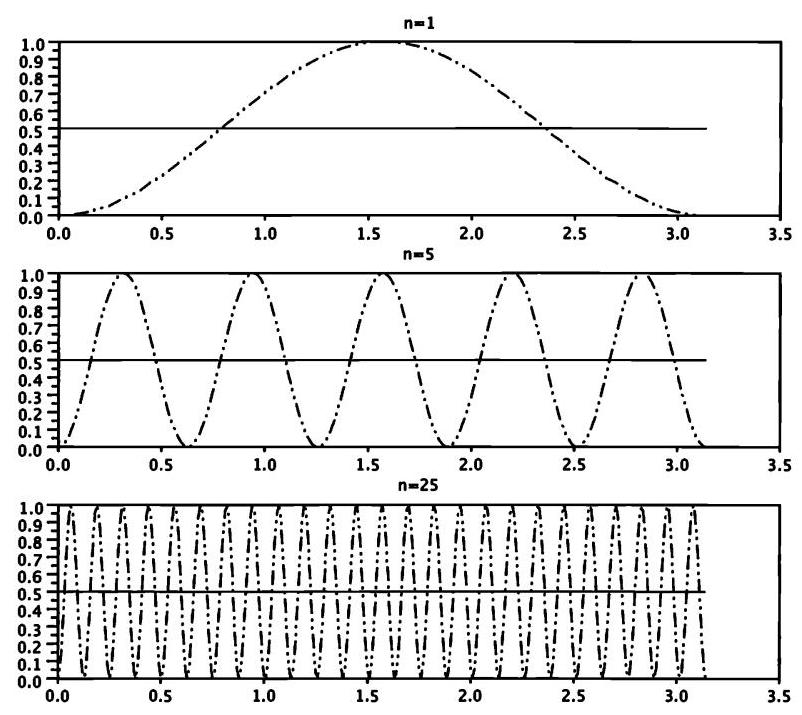
\includegraphics[width=0.7\textwidth]{images/bo_d6ik6nn7aajc739ct1l0_106_338_561_802_715_0.jpg}
\caption{函数 ${f}_{n}\left( x\right)  = {\sin }^{2}{nx}$ 的图像( $n =$ 取1、5、25).当 $n \rightarrow  \infty$ 时，函数 ${f}_{n}$ 既不逐点收敛，也不按 ${L}^{2}$ 范数收敛.然而，我们有弱收敛 ${f}_{n} \rightharpoonup \; f \equiv  1/2$ ，因为 ${f}_{n}$ 在任意区间 $\left(  {a,b}\right)$ 上的平均值均收敛于常数 $1/2$ .}\label{fig:weak-convergence-sin2nx}
\end{figure}

\begin{instance}\label{ins:weak-convergence-sin2nx}
在空间 ${L}^{2}\left( \left(  {0,\pi }\right)  \right)$ 中，考虑函数列 ${f}_{n}\left( x\right)  = {\sin }^{2}{nx}$ (见图\ref{fig:weak-convergence-sin2nx}).我们断言该函数列弱收敛于常值函数 $f\left( x\right)  \equiv  1/2$ .事实上，对任意 $g \in \; {L}^{2}\left( \left(  {0,\pi }\right)  \right)$ ，需证明
\begin{equation}\tag{5.26}\label{eq:weak-sin2nx-mean}
\mathop{\lim }\limits_{{n \rightarrow  \infty }}{\int }_{0}^{\pi }g\left( x\right) {\sin }^{2}\left( nx\right) \,dx = {\int }_{0}^{\pi }\frac{g\left( x\right) }{2}\,dx.
\end{equation}

在如下特殊情形下
\begin{equation}\tag{5.27}\label{eq:step-function-example}
g\left( x\right)  = \begin{cases}
1, & \text{ if }x \in  \left(  {0,b}\right), \\
0, & \text{ if }x \in  \left( b,\pi \right).
\end{cases}
\end{equation}

结论显然成立，因为
\[
\mathop{\lim }\limits_{{n \rightarrow  \infty }}{\int }_{0}^{b}{\sin }^{2}{nxdx} = \mathop{\lim }\limits_{{n \rightarrow  \infty }}\left( {\frac{b}{2} - \frac{\sin {2nb}}{4n}}\right)  = \frac{b}{2} = {\int }_{0}^{\pi }\frac{g\left( x\right) }{2}{dx}.
\]

由线性性可知，\eqref{eq:weak-sin2nx-mean}式对形如\eqref{eq:step-function-example}的函数的所有线性组合——即对所有分段常值函数——均成立.

现考虑任意函数 $g \in  {L}^{2}$ .对任意 $\varepsilon  > 0$ ，可找到一分段常值函数 $\widetilde{g}$ ，使得 $\| g - \widetilde{g}{\| }_{{L}^{2}} < \varepsilon$ .由此可得
\begin{align*}
    &{\int }_{0}^{\pi }g\left( x\right) \left( {{\sin }^{2}{nx} - \frac{1}{2}}\right) {\d x}\\
    &= {\int }_{0}^{\pi }\widetilde{g}\left( x\right) \left( {{\sin }^{2}{nx} - \frac{1}{2}}\right) {\d x} + {\int }_{0}^{\pi }\left(  {\widetilde{g}\left( x\right)  - g\left( x\right) }\right)   \cdot  \left( {{\sin }^{2}{nx} - \frac{1}{2}}\right) {\d x}\\
    &\doteq  {A}_{n} + {B}_{n}.
\end{align*}

由于 $\widetilde{g}$ 是分段常值函数，我们已知当 $n \rightarrow  \infty$ 时， ${A}_{n} \rightarrow  0$ .另一方面，由Cauchy不等式，
\[
\left| {B}_{n}\right|  \leq  \| \widetilde{g} - g{\| }_{{L}^{2}} \cdot  {\left( {\int }_{0}^{\pi }{\left( {\sin }^{2}nx - \frac{1}{2}\right) }^{2}\ d x\right) }^{1/2} < \varepsilon  \cdot  {\left( \frac{\pi }{4}\right) }^{1/2}.
\]

因 $\varepsilon$ 可任取充分小，故证得弱收敛 ${f}_{n} \rightharpoonup  f$ .

注意强收敛并不成立.事实上，
\[
\mathop{\lim }\limits_{{n \rightarrow  \infty }}{\norm{f}_{n} - f}_{{L}^{2}}^{2} = \mathop{\lim }\limits_{{n \rightarrow  \infty }}{\int }_{0}^{\pi }{\left( {\sin }^{2}nx - \frac{1}{2}\right) }^{2}{\d x} = \frac{1}{8}.
\]

接下来，考虑由 ${L}^{2}\left( \left(  {0,\pi }\right)  \right)$ 到其自身的紧算子 $\Lambda$ ，定义为
\[
\left( {\Lambda g}\right) \left( x\right)  \doteq  {\int }_{0}^{x}g\left( y\right) {\d y}.
\]

该积分算子将序列 ${f}_{n}\left( x\right)  = {\sin }^{2}{nx}$ 映为序列
\[
\left( {\Lambda {f}_{n}}\right) \left( x\right)  = {\int }_{0}^{x}{\sin }^{2}{ny\d y} = \frac{x}{2} - \frac{\sin {2nx}}{4n}.
\]

此外， $\left( {\Lambda f}\right) \left( x\right)  = x/2$ .注意到 $\Lambda {f}_{n}$ 在 $\left(  {0,\pi }\right)$ 上一致收敛于 ${\Lambda f}$ .特别地，我们有强收敛 $\| \Lambda {f}_{n} - {\Lambda f}{\| }_{{L}^{2}} \rightarrow  0$ .这为定理\ref{thm:compact-weak-to-strong}提供了例证:紧算子将弱收敛序列映为强收敛序列.
\end{instance}

\section{习题}

\begin{rbhw}[index=1]
设 $H$ 为Hilbert空间.利用内积定义，证明\eqref{eq:inner-product-linearity}中的两个恒等式；并证明勾股定理:若两向量 $x,y \in  H$ 彼此正交，则 $\| x{\| }^{2} + \| y{\| }^{2} = \| x + y{\| }^{2}$ .
\end{rbhw}

\begin{rbhw}
设 $H$ 为具内积 $\left( {\cdot , \cdot  }\right)$ 的向量空间.证明内积是从积空间 $H \times  H$ 到 $\mathbb{K}$ 的连续映射.换言之，若 ${x}_{k} \rightarrow  x$ 且 ${y}_{k} \rightarrow  y$ (按范数\eqref{eq:norm-from-inner-product})，则内积序列 $\left( {{x}_{k},{y}_{k}}\right)$ 收敛于 $\left( {x,y}\right)$.在 $H \times  H$ 上考虑范数 $\| \left( {x,y}\right) \|  \doteq  {\left( \| x{\| }^{2} + \| y{\| }^{2}\right) }^{1/2}$ .
\end{rbhw}

\begin{rbhw}
设 $X$ 为实数域上的Banach空间，其范数为 $\|  \cdot  \|$ .是否存在 $X$ 上的内积 $\left( {\cdot , \cdot  }\right)$ ，使得对每个 $x \in  X$ 均有 $\| x\|  = \sqrt{\left( x,x\right) }$ ？请按以下两个步骤作答.
(i) 设 $H$ 为实Hilbert空间.证明其范数 $\| x\|  = \sqrt{\left( x,x\right) }$ 满足平行四边形恒等式\eqref{eq:parallelogram-identity}
\begin{equation}\tag{5.28}\label{eq:parallelogram-identity}
\| x + y{\| }^{2} + \| x - y{\| }^{2} = 2\| x{\| }^{2} + 2\| y{\| }^{2}\;\forall\,x,y \in  X.
\end{equation}
(ii) 反之，设 $X$ 为实数域上的Banach空间，且其范数满足平行四边形恒等式\eqref{eq:parallelogram-identity}.证明
\[
\left( {x,y}\right)  \doteq  \frac{1}{2}\left( {\| x + y{\| }^{2} - \| x{\| }^{2} - \| y{\| }^{2}}\right)  = \frac{1}{4}\left( {\| x + y{\| }^{2} - \| x - y{\| }^{2}}\right)
\]

是 $X$ 上的一个内积，且恰好给出范数 $\|  \cdot  \|$ .提示:为证明 $\left( {x + {x}^{\prime },y}\right)  = \left( {x,y}\right)  + \left( {{x}^{\prime },y}\right)$ ，首先建立恒等式
\[
{\norm{x} + {x}^{\prime } + y}^{2} = {\norm{x}}^{2} + {\norm{x}^{\prime }}^{2} + \| x + y{\| }^{2} + {\norm{x}^{\prime } + y}^{2} - \frac{1}{2}{\norm{x} + y - {x}^{\prime }}^{2} - \frac{1}{2}{\norm{x}^{\prime } + y - x}^{2}.
\]

为证明 $\left( {{\lambda x},y}\right)  = \lambda \left( {x,y}\right)$ ，先验证该恒等式在 $\lambda$ 为整数时成立，再推广至 $\lambda$ 为有理数的情形，最后由连续性推广至所有 $\lambda  \in  \mathbb{R}$ .
\end{rbhw}

\begin{rbhw}
利用上述问题，证明:

(i) 在向量空间 ${\mathbb{R}}^{2}$ 上，对所有满足 $p \neq  2$ 的 $p \geq  1$ ，范数 $\| \bm{x}{\| }_{p} \doteq  \left( {{\left| {x}_{1}\right| }^{p} + }\right. \; {\left. {\left| {x}_{2}\right| }^{p}\right) }^{1/p}$ 不能由内积生成.

(ii) 在实值连续函数空间 $\mathcal{C}\left( \left(  {0,1}\right)  \right)$ 上，范数 $\| f\|  \doteq \; \mathop{\max }\limits_{{x \in  \left(  {0,1}\right)  }}\left| {f\left( x\right) }\right|$ 不能由内积生成.
\end{rbhw}

\begin{rbhw}
考虑Hilbert空间 $H = {L}^{2}\left( \left(  {-1,1}\right)  \right)$ ，其内积为 $\left( {f,g}\right)  = \; {\int }_{-1}^{1}{fgdx}$ .证明多项式序列 $\left\{  {1,x,{x}^{2},{x}^{3},\ldots }\right\}$ 线性无关，且其张成空间在 $H$ 中稠密.应用Gram-Schmidt正交化过程，构造一组标准正交多项式序列 $\left\{  {{p}_{0},{p}_{1},{p}_{2},{p}_{3},\ldots }\right\}$ (与勒让德多项式成比例).显式计算前三个多项式.
\end{rbhw}

\begin{rbhw}
设 ${\left( {e}_{n}\right) }_{n \geq  1}$ 为Hilbert空间 $H$ 中的一组标准正交序列.证明弱收敛 ${e}_{n} \rightharpoonup  0$ .即证明:对每个 $x \in  H$ ，均有 $\mathop{\lim }\limits_{{n \rightarrow  \infty }}\left( {x,{e}_{n}}\right)  = 0.$
\end{rbhw}

\begin{rbhw}
设 $H$ 为无限维Hilbert空间，给定任意向量 $x \in  H$ ，满足 $\| x\|  \leq  1$ .构造向量序列 ${x}_{n}$ ，使得对每个 $n \geq  1$ 均有 $\norm{x}_{n} = 1$ ，且弱收敛成立: ${x}_{n} \rightharpoonup  x$ .
\end{rbhw}

\begin{rbhw}
设 ${\left( {v}_{k}\right) }_{k \geq  1}$ 为实Hilbert空间 $H$ 中的一列单位向量， ${\left( {\alpha }_{k}\right) }_{k \geq  1}$ 为一列实数.

(i) 若 $\sum\limits_{{k = 1}}^{\infty }\left| {\alpha }_{k}\right|  < \infty$ ，证明级数 $\sum\limits_{{k = 1}}^{\infty }{\alpha }_{k}{v}_{k}$ 收敛.

(ii) 假设序列 ${\left( {v}_{k}\right) }_{k \geq  1}$ 标准正交.此时证明:级数 $\sum\limits_{{k = 1}}^{\infty }{\alpha }_{k}{v}_{k}$ 收敛当且仅当 $\sum\limits_{{k = 1}}^{\infty }{\left| {\alpha }_{k}\right| }^{2} < \infty$ .
\end{rbhw}

\begin{rbhw}
设 $\phi  : {\mathbb{R}}^{n} \mapsto  {\mathbb{R}}^{n}$ 为光滑双射，且雅可比矩阵的行列式对所有 $x \in  {\mathbb{R}}^{n}$ 满足 $\det {D\phi }\left( x\right)  = 1$ ，从而 $\phi$ 保体积.在空间 ${L}^{2}\left( {\mathbb{R}}^{n}\right)$ 上考虑线性算子 $\left( {\Lambda f}\right) \left( x\right)  \doteq  f\left( {\phi \left( x\right) }\right)$ .证明:
\[
\| \Lambda \|  = 1,\;{\Lambda }^{ * } = {\Lambda }^{-1}.
\]

注意， $\Lambda$ 可视为空间 ${L}^{2}\left( {\mathbb{R}}^{n}\right)$ 中的一个旋转，因为其伴随算子等于其逆算子.
\end{rbhw}

\begin{rbhw}
考虑Hilbert空间 ${\ell }^{2}$ ，即所有满足 $\sum\limits_{{k = 1}}^{\infty }{\left| {x}_{k}\right| }^{2} < \infty$ 的实数列 $\bm{x} = \left( {{x}_{1},{x}_{2},\ldots }\right)$ 构成的空间，其内积为 $\left( {\bm{x},\bm{y}}\right)  \doteq  \sum\limits_{{k = 1}}^{\infty }{x}_{k}{y}_{k}$ .定义算子 $\Lambda  : H \mapsto  H$ 如下: $\Lambda \left( {{x}_{1},{x}_{2},{x}_{3},\ldots }\right)  \doteq  \left( {{x}_{2},{x}_{3},{x}_{4},\ldots }\right)$ .计算其伴随算子 ${\Lambda }^{ * }$ .算子 $\Lambda ,{\Lambda }^{ * }$ 是否满射？是否单射？
\end{rbhw}

\begin{rbhw}
设 $S$ 为凸集.称 $x \in  S$ 是 $S$ 的一个极点，若 $x$ 不能表示为 $S$ 中两个不同点的凸组合.换言之，
\[
x \neq  \theta {x}_{1} + \left( {1 - \theta }\right) {x}_{2}\;\text{当}\; 0 < \theta  < 1,\;{x}_{1},{x}_{2} \in  S,\;{x}_{1} \neq  {x}_{2}.
\]

证明以下结论.

(i) 若 $S$ 是Hilbert空间 $H$ 中的闭单位球，则对任意满足 $\| x\|  = 1$ 的点 $x \in  S$ ，它都是 $S$ 的一个极点.特别地，这对空间 $H = {L}^{2}\left( \left(  {0,1}\right)  \right)$ 成立.

(ii) 另一方面，考虑 ${L}^{1}\left( \left(  {0,1}\right)  \right)$ 中的单位球，即
\[
B \doteq  \left\{  {f : \left(  {0,1}\right)   \mapsto  \mathbb{R};{\int }_{0}^{1}\left| {f\left( t\right) }\right| {dt} \leq  1}\right\}  .
\]

证明 $B$ 不包含任何极点.
\end{rbhw}

\begin{rbhw}
设 ${\left( {x}_{n}\right) }_{n > 1}$ 是Hilbert空间 $H$ 中的一列点，满足 $C \doteq \; \mathop{\liminf }\limits_{{n \rightarrow  \infty }}\norm{x}_{n} < \infty$ .证明存在一个弱收敛子列 ${x}_{{n}_{j}} \rightharpoonup  x$ ，其中某点 $x \in  H$ 满足 $\| x\|  \leq  C$ .
\end{rbhw}

\begin{rbhw}
设 $H$ 是一个无限维、可分的实Hilbert空间， ${\ell }^{2}$ 是所有满足 $\| \bm{a}{\| }_{{\ell }^{2}} \doteq \; {\left( \sum\limits_{{k = 1}}^{\infty }{a}_{k}^{2}\right) }^{1/2} < \infty$ 的实数列 $\bm{a} = \left( {{a}_{1},{a}_{2},\ldots }\right)$ 构成的空间.构造一个保距线性双射 $\Lambda  : H \mapsto  {\ell }^{2}$ ，即满足
\[
\| {\Lambda x}{\| }_{{\ell }^{2}} = \| x{\| }_{H}\;\forall\,x \in  H.
\]
\end{rbhw}

\begin{rbhw}
给定实Hilbert空间 $H$ 中的 $n$ 个向量 ${v}_{1},{v}_{2},\ldots ,{v}_{n}$ ，将其Gram行列式定义为\eqref{eq:gram-schmidt-linear-system}式中 $n \times  n$ 阶对称矩阵的行列式:
\[
G\left( {{v}_{1},\ldots ,{v}_{m}}\right)  \doteq  \det \left( \begin{matrix} \left( {{v}_{1},{v}_{1}}\right) & \cdots & \left( {{v}_{n},{v}_{1}}\right) \\  \vdots &  \ddots  & \vdots \\  \left( {{v}_{1},{v}_{n}}\right) & \cdots & \left( {{v}_{n},{v}_{n}}\right)  \end{matrix}\right) .
\]

(i) 利用\eqref{eq:gram-schmidt-linear-system}并取 $x = 0$ ，证明向量 ${v}_{1},\ldots ,{v}_{n}$ 线性无关当且仅当 $G\left( {{v}_{1},\ldots ,{v}_{n}}\right)  \neq  0$ .

(ii) 假设向量 ${v}_{1},\ldots ,{v}_{n}$ 线性无关，考虑子空间 $V \doteq  \operatorname{span}\left\{  {{v}_{1},\ldots ,{v}_{n}}\right\}$ .对任意向量 $x \in  H$ ，证明 $x$ 到 $V$ 的距离为
\[
d\left( {x,V}\right)  = \norm{x - {P}_{V}\left( x\right) } = \sqrt{\frac{G\left( {x,{v}_{1},{v}_{2},\ldots ,{v}_{n}}\right) }{G\left( {{v}_{1},{v}_{2},\ldots ,{v}_{n}}\right) }}.
\]

(iii) 如图\ref{fig:gram-determinant-parallelepiped}所示，证明以 ${v}_{1},\ldots ,{v}_{n}$ 为棱的 $n$ 维平行多面体的体积可表示为
\[
\norm{v}_{1} \cdot  d\left( {{v}_{2};\operatorname{span}\left\{  {v}_{1}\right\}  }\right)  \cdot  d\left( {{v}_{3};\operatorname{span}\left\{  {{v}_{1},{v}_{2}}\right\}  }\right) \cdots d\left( {{v}_{n};\operatorname{span}\left\{  {{v}_{1},\ldots ,{v}_{n - 1}}\right\}  }\right) .
\]

利用 (ii)，证明该平行多面体的体积为 $\sqrt{G\left( {{v}_{1},{v}_{2},\ldots ,{v}_{n}}\right) }$ .

\begin{figure}[htbp]
\centering
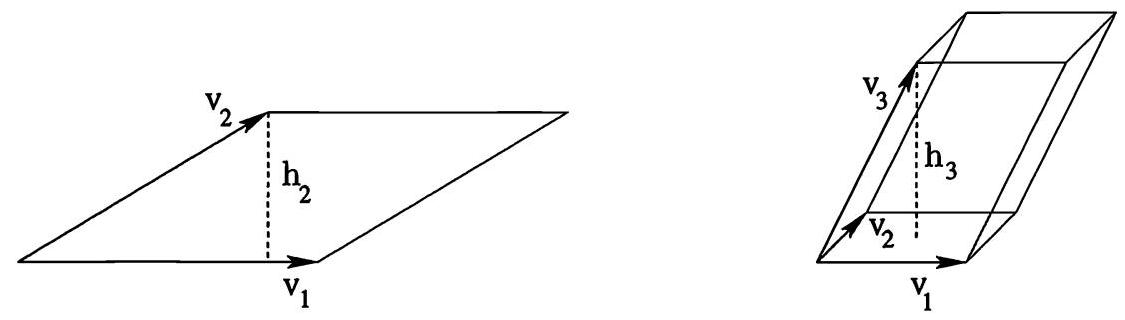
\includegraphics[width=\textwidth]{images/bo_d6ik6nn7aajc739ct1l0_110_169_1151_1125_320_0.jpg}
\caption{计算平行四边形面积与平行多面体体积.此处 ${h}_{2} = d\left( {{v}_{2},\operatorname{span}\left\{  {v}_{1}\right\}  }\right)$ ，而 ${h}_{3} = d\left( {{v}_{3},\operatorname{span}\left\{  {{v}_{1},{v}_{2}}\right\}  }\right) .$}\label{fig:gram-determinant-parallelepiped}
\end{figure}
\end{rbhw}

\begin{rbhw}
设 $f \in  {L}^{2}\left( \mathbb{R}\right)$ .证明存在唯一的偶\footnote{偶函数是指满足 $f(-x) = f(x)$ 的函数}函数 ${g}_{0}$ ，使得
\[
{\norm{f} - {g}_{0}}_{{L}^{2}} = \mathop{\min }\limits_{{g \in  {L}^{2}\left( \mathbb{R}\right) ,g\text{ even }}}\| f - g{\| }_{{L}^{2}}.
\]

显式确定函数 ${g}_{0}$ .
\end{rbhw}

\begin{rbhw}
设 $K \in  \mathcal{B}\left( {X;H}\right)$ 是从 Banach 空间 $X$ 到 Hilbert 空间 $H$ 的有界线性算子.证明下列条件等价.

(i) $K$ 是紧算子.

(ii) 对每个 $\varepsilon  > 0$ ，存在一个具有有限维值域的算子 ${K}_{\varepsilon } : X \mapsto  H$ ，使得 $\norm{{K}_{\varepsilon } - K} < \varepsilon$ .
\end{rbhw}

\begin{rbhw}
设 ${\left\{  {u}_{n}\right\}  }_{n \geq  1}$ 和 ${\left\{  {v}_{n}\right\}  }_{n \geq  1}$ 是 Hilbert 空间 $H$ 中的两个标准正交集.假设
\[
\sum\limits_{{n = 1}}^{\infty }\norm{{u}_{n} - {v}_{n}} < 1
\]

证明:若其中一个集合是完备的，则另一个集合也完备.
\end{rbhw}

\begin{rbhw}
设 $\left\{  {{u}_{n};n \geq  1}\right\}$ 是 Hilbert 空间 $H$ 中一组可数的线性无关单位向量.考虑向量 $v \doteq  \sum\limits_{{n = 1}}^{\infty }{2}^{-n}{u}_{n}$ .

(i) 假设所有向量 ${u}_{n}$ 两两正交，证明集合 $S \doteq  \left\{  {v,{u}_{1},{u}_{2},{u}_{3},\ldots }\right\}$ 线性无关.

(ii) 举一反例说明:若向量 ${u}_{n}$ 并非两两正交，则上述集合 $S$ 可能线性相关.
\end{rbhw}

\begin{rbhw}
给定 Hilbert 空间 $H$ 中的序列 ${\left( {x}_{n}\right) }_{n \geq  1}$ ，证明强收敛 $\norm{{x}_{n} - x} \rightarrow  0$ 成立当且仅当
\[
\norm{x}_{n} \rightarrow  \| x\| \;\text{ and }\;{x}_{n} \rightharpoonup  x\text{ (弱收敛). }
\]
\end{rbhw}

\begin{rbhw}
设 $Q = \left(  {0,1}\right)   \times  \left(  {0,1}\right)$ 为单位正方形.在空间 ${L}^{2}\left( Q\right)$ 中，考虑仅依赖于变量 $y$ 的所有函数构成的子空间:
\[
U = \left\{  {u \in  {L}^{2}\left( Q\right) ;\exists\,\varphi  : \left(  {0,1}\right)   \mapsto  \mathbb{R},u\left( {x,y}\right)  = \varphi \left( y\right)},\,\text{a.e.}\,{\left( {x,y}\right)  \in  Q}\right\}  \text{ . }
\]
(i) 求正交补子空间 $W = {U}^{ \bot  }$ .

(ii) 对任意 $f \in  {L}^{2}\left( Q\right)$ ，确定函数 $g \in  U$ ，使得
\[
\| f - g{\| }_{{L}^{2}\left( Q\right) } = \mathop{\min }\limits_{{u \in  U}}\| f - u{\| }_{{L}^{2}\left( Q\right) }.
\]
\end{rbhw}

\begin{rbhw}
设 $H$ 是 Hilbert 空间， $\Omega  \subset  H$ 是其闭凸子集.

(i) 证明:对任意 $x \in  H$ ，存在唯一一点 $y \in  \Omega$ ，使得 $\| y - x\|  = \mathop{\min }\limits_{{\omega  \in  \Omega }}\| \omega  - x\|$ .该最小距离点 $y = {\pi }_{\Omega }\left( x\right)$ 称为 $x$ 到 $\Omega$ 的垂足投影.

(ii) 证明: $y = {\pi }_{\Omega }\left( x\right)$ 当且仅当 $\langle \omega  - y,y - x) \geq  0$ 对所有 $\omega  \in  \Omega$ 成立.
\end{rbhw}

\begin{rbhw}
在Hilbert空间 $H = {L}^{2}\left( \mathbb{R}\right)$ 上，考虑子集
\[
\Omega  \doteq  \left\{  {f;f\left( x\right)  \leq  {e}^{x}\text{ for a.e. }x \in  \mathbb{R}}\right\}  .
\]

(i) 证明 $\Omega$ 是 $H$ 的闭凸子集.

(ii) 证明到 $\pi  : H \mapsto  \Omega$ 的正交投影即为定义为 $\left( {\pi f}\right) \left( x\right)  = \min \left\{  {f\left( x\right) ,{e}^{x}}\right\}  .$ 的映射.
\end{rbhw}

\begin{rbhw}
在Hilbert空间 $H = {L}^{2}\left( \mathbb{R}\right)$ 上，考虑由 $\left( {\Lambda f}\right) \left( x\right)  = f\left( \left| x\right| \right)$ 定义的线性算子 $\Lambda  : H \mapsto  H$ .

(i) 求 $\Lambda$ 的算子范数.

(ii) 求 $\Lambda$ 的核与值域.

(iii) 计算 ${\Lambda }^{ * }$ 的伴随算子.
\end{rbhw}

\begin{rbhw}
在Hilbert空间 $H = {L}^{2}\left( \left(  {0,\infty }\right)  \right)$ 上，考虑线性算子 $\left( {\Lambda f}\right) \left( x\right)  = f\left( {e}^{x}\right)$ .

(i) 计算线性算子 $\Lambda$ 的范数.

(ii) 求 $\Lambda$ 的核与值域.

(iii) 计算 ${\Lambda }^{ * }$ 的伴随算子.
\end{rbhw}

\begin{rbhw}
考虑函数列 ${f}_{n} \in  {L}^{2}\left( \left(  {0,T}\right)  \right)$ 的有界性.当 $n \rightarrow  \infty$ 时，证明弱收敛 ${f}_{n} \rightharpoonup  f$ 成立当且仅当
\[
\mathop{\lim }\limits_{{n \rightarrow  \infty }}{\int }_{0}^{b}{f}_{n}\left( x\right) {dx} = {\int }_{0}^{b}f\left( x\right) {dx}\;\text{ for every }b \in  \left(  {0,T}\right)  .
\]
\end{rbhw}

\begin{rbhw}
在空间 ${L}^{2}\left( \left(  {0,1}\right)  \right)$ 上，考虑如下两列函数
\[
{f}_{n}\left( x\right)  = \sqrt{n} \cdot  \cos {nx},\;{f}_{n}\left( x\right)  = \left\{  \begin{matrix} {n}^{2/3} & \text{ if } & x \in  \left(  {0,{n}^{-1}}\right)  , \\  0 & \text{ if } & x > {n}^{-1}. \end{matrix}\right.
\]

(i) 两种情形下，均证明对每个 $b \in  \left(  {0,1}\right)$ 有 $\mathop{\lim }\limits_{{n \rightarrow  \infty }}{\int }_{0}^{b}{f}_{n}\left( x\right) {dx} = 0$ .

(ii) 通过取线性组合，证明对每个分段常值函数 $g$ 有 $\mathop{\lim }\limits_{{n \rightarrow  \infty }}{\int }_{0}^{1}{f}_{n}{gdx} = 0$ .

(iii) 是否成立 ${f}_{n} \rightharpoonup  0$ ？
\end{rbhw}

\begin{rbhw}
设 ${\left( {x}_{n}\right) }_{n \geq  1}$ 是Hilbert空间 $H$ 中的一个序列，证明下列命题等价.

(i) 弱收敛成立: ${x}_{n} \rightharpoonup  x$ .

(ii) 序列 $\left( {x}_{n}\right)$ 有界，且对某个具有非空内部闭包的子集 $S \subseteq  H$ 中的所有 $y$ 均有 $\left( {y,{x}_{n}}\right)  \rightarrow  \left( {y,x}\right)$ .
\end{rbhw}

\begin{rbhw}
设 $\Omega  \subseteq  {\mathbb{R}}^{N}$ 为开集.证明函数列 ${f}_{n} \in  {L}^{2}\left( \Omega \right)$ 弱收敛于 $f$ 当且仅当存在常数 $C$ ，使得对每个 $n \geq  1$ 均有 ${\norm{f}_{n}}_{{L}^{2}} \leq  C$ ，且此外
\[
\mathop{\lim }\limits_{{n \rightarrow  \infty }}{\int }_{Q}{f}_{n}{dx} = {\int }_{Q}{fdx}
\]

对每个完全包含于 $\Omega$ 中的矩形 $Q = \left(  {{a}_{1},{b}_{1}}\right)   \times  \left(  {{a}_{2},{b}_{2}}\right)   \times  \cdots  \times  \left(  {{a}_{N},{b}_{N}}\right)$ 均成立.
\end{rbhw}

\begin{rbhw}
在实Hilbert空间 $H$ 中，考虑弱收敛序列: ${x}_{n} \rightharpoonup  y$ .令 $S \doteq  \overline{\operatorname{co}\left\{  {{x}_{n};n \geq  1}\right\}  }$ 为包含所有点 ${x}_{n}$ 的最小闭凸集.证明 $y \in  S$ .
\end{rbhw}